%! Author = Miriam Streit
%! Date = 17.06.23

\section{Laufzeitsicht}
\label{sec:laufzeitsicht}
In diesem Kapitel wird die Laufzeitsicht der Anwendung beschrieben. Es wird aufgezeigt, wie die verschiedenen Komponenten der Anwendung zur Laufzeit zusammenarbeiten.

\subsection{Bestellung aufgeben}
\label{subsec:bestellung-aufgeben}
Bei einer neuen Bestellung werden mehrere Schritte im Hintergrund ausgeführt. Zuerst wird die Bestellung im Frontend aufgegeben. Das Frontend sendet zuerst eine Anfrage an den Customer-Service mit den Personal-Daten des Bestellers. Der Customer-Service überprüft an hand von Vorname, Nachname und Adresse, ob dieser Customer bereits existiert. Falls nicht, wird ein neuer Customer erstellt. Anschliessend wird die Customer-Id zurück an das Frontend gesendet. Das Frontend sendet nun eine Anfrage an den Order-Service mit Customer-Id, Biersorten-Id's und Menge pro Sorte. Der Order-Service kann nun mit Hilfe der Biersorten-Id's die Preise der Sorten in der Datenbank abfragen. Zusammen mit Preis und Menge pro Sorte kann nun der Gesamtpreis berechnet werden. Zuletzt wird die Bestellung in der Datenbank gespeichert. Die Abbildung \ref{fig:bestellung-aufgeben} zeigt diesen Ablauf.

\begin{figure}[H]
    \centering
    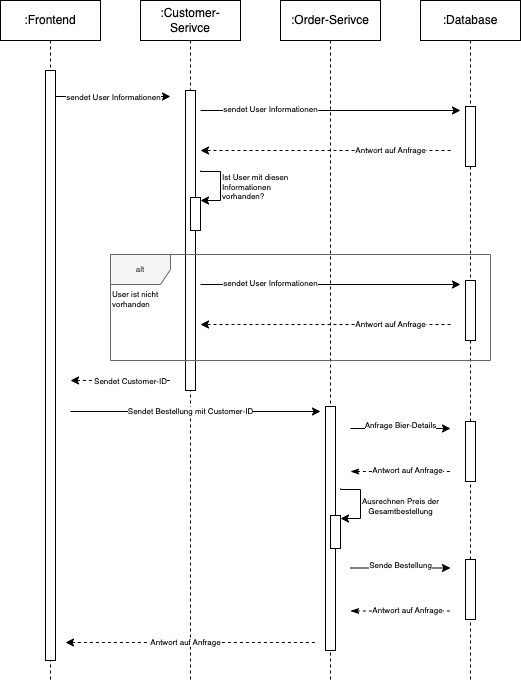
\includegraphics[width=0.7\textwidth]{images/laufzeitsicht_bestellung.png}
    \caption{Sequenzdiagramm Bestellung aufgeben}
    \label{fig:bestellung-aufgeben}
\end{figure}
